%%%%%%%%%%%%%%%%%%%%%%%%%%%%%%%%%%%%%%%%%%%%%%%%%%%%%%%%%%%%%%%%%%%%%%%%%%%%%%%%
%2345678901234567890123456789012345678901234567890123456789012345678901234567890
%        1         2         3         4         5         6         7         8

\documentclass[letterpaper, 10 pt, conference]{ieeeconf}  % Comment this line out if you need a4paper

%\documentclass[a4paper, 10pt, conference]{ieeeconf}      % Use this line for a4 paper

\IEEEoverridecommandlockouts                              % This command is only needed if 
                                                          % you want to use the \thanks command

\overrideIEEEmargins                                      % Needed to meet printer requirements.

\usepackage{cite}
\usepackage{amsmath,amssymb,amsfonts}
\usepackage{algorithmic}
\usepackage{graphicx}
\usepackage{textcomp}
\usepackage{amsmath}
\usepackage{stfloats}
\usepackage[]{algorithm2e}
\usepackage{subcaption,siunitx,booktabs}

\usepackage{tabularx, booktabs} 
\def\BibTeX{{\rm B\kern-.05em{\sc i\kern-.025em b}\kern-.08em
    T\kern-.1667em\lower.7ex\hbox{E}\kern-.125emX}}
\graphicspath{{./images/}}
\newcolumntype{C}{>{\centering\arraybackslash}p{1.8cm}}
\usepackage{hyperref}
\hypersetup{pdftex,colorlinks=true,allcolors=blue}
\usepackage{hypcap}
%In case you encounter the following error:
%Error 1010 The PDF file may be corrupt (unable to open PDF file) OR
%Error 1000 An error occurred while parsing a contents stream. Unable to analyze the PDF file.
%This is a known problem with pdfLaTeX conversion filter. The file cannot be opened with acrobat reader
%Please use one of the alternatives below to circumvent this error by uncommenting one or the other
%\pdfobjcompresslevel=0
%\pdfminorversion=4

% See the \addtolength command later in the file to balance the column lengths
% on the last page of the document

% The following packages can be found on http:\\www.ctan.org
%\usepackage{graphics} % for pdf, bitmapped graphics files
%\usepackage{epsfig} % for postscript graphics files
%\usepackage{mathptmx} % assumes new font selection scheme installed
%\usepackage{times} % assumes new font selection scheme installed
%\usepackage{amsmath} % assumes amsmath package installed
%\usepackage{amssymb}  % assumes amsmath package installed

\title{\LARGE \bf
WARWICK algorithm for separating recurrent and outstanding congestion in Motorways and long-term travel time forecasting*
}


\author{Alvaro Cabrejas Egea$^{1}$ and Colm Connaughton$^{2}$% <-this % stops a space
\thanks{*This work was part funded by the EPSRC under grant no. EP/L015374.}% <-this % stops a space
\thanks{$^{1}$Alvaro Cabrejas Egea is with MathSys Centre for Doctoral Training, University of Warwick, CV4 7AL, Coventry, United Kingdom and The Alan Turing Institute, NW1 2DB, London, United Kingdom
        {\tt\small a.cabrejas-egea@warwick.ac.uk}}%
\thanks{$^{2}$ Colm Connaughton with the Warwick Mathematics Institute \& Centre for Complexity Science, University of Warwick,
        CV4 7AL, Coventry, United Kingdom
        {\tt\small c.p.connaughton@warwick.ac.uk}}%        
}


\begin{document}



\maketitle
\thispagestyle{empty}
\pagestyle{empty}


\begin{abstract}
We present the new WARWICK method for separating recurrent and outstanding congestion from a travel time time series using wavelets. 
We train and test this method using 12 weeks of real time travel data gathered at link level in the M6 and M11 in the United Kingdom.
The approach is based on a time travel series analysis of travel time data from the UK's National Traffic Information Service (NTIS).
Time series of travel times are characterised by a noisy background component showing the expected seasonal patterns and occasional large spikes associated with congestion events.
The separation algorithm here presented uses statistical analysis of the Wavelet Transform of the travel times across different time scales to split the original signal into two signals in the time-frequency domain: background and spikes, and then inverse transform them to use them for forecasting.
We process and combine 8 weeks of these signals, using spectral filtering and non-parametric locally weighted regression (LWR) to predict travel time in the link in the following week with a resolution of one minute, repeating this process 4 times on a rolling basis.
We find that the error is meaningfully reduced compared to estimates obtained by basic time segmentation of the data and compared to the estimates published by the NTIS system.

Wavelet
Augmented
Regression
With
spIkes and
baCKground

\end{abstract}

\section{Introduction} \label{Introduction}
\subsection{Background} \label{Background}
Incident detection algorithms yield a large number of false alarms and missed detections. This is mainly
due to random temporal fluctuations or traffic noise that
makes it difficult to differentiate between recurrent and
non-recurrent congestion accurately

Highways England (HE) is responsible for most Motorways and major roads in England, comprising the Strategic Road Network (SRN).
The SRN is monitored by the National Traffic Information System \cite{NTIS}, which collects and processes travel time, speed, flow and overhead space data in real time using sensors on the road and in vehicles.
The smallest components of the SRN are the so called links, which are segments of motorway between 500 and 20000 metres in length.
NTIS uses the historic series of real time logged data to assign each link in the network with a traffic profile.
Traffic profiles contain, for each minute of a day in a given date, the expected travel time to transverse the link to which it is associated. 
These profile values are published together with the measured travel times, but the methodology followed to calculate them is not publicly available.

While the profiles, in fairly used roads, vary with the day of the week and time of the day, their inter-week variation remains low, with major trends changes taking longer (order of months) than the biggest temporal unit considered (weeks). 
This display of stability over time, means that calculating profiles is a different problem when compared with short-term forecasting.
Since there is no a-priori mathematical definition of typical travel times, here, we will take it as the value that minimises the Mean Absolute Relative Error (MARE) or Root Mean Squared Error (RMSE), when comparing it with the subsequently sampled real travel times.

\subsection{Previous Work} \label{Previous Work}
In this paper, we follow up on the future work indicated in \cite{ttprofiles}, aiming to provide with a novel algorithm that outputs one week of expected travel times, removing the heuristically set threshold in said paper.

Our approach is based on statistical analysis of previous data and does not require any a-priori segmentation of days into classes. 
Rather, the algorithm relies on patterns of intra- and inter-day variability which are learned from input data.

The Continuous Wavelet Transform \cite{morletwavelet}


***
The available literature on travel times is extensive but most recent research focuses on short-term forecasting and with fewer studies looking into the long term \cite{long-term} \cite{long-term-2}. 
From a methodological point of view statistical methods and machine learning take most of the attention \cite{should}. Within the last group, neural networks are getting a level or relevance \cite{NN} \cite{spectral2} .
Others take closer approaches to this paper: using historical data \cite{simple} \cite{dynamic-historic}, differentiating between peak and non-peak \cite{peak-historic}, performing spectral analysis \cite{spectral1} or Locally Weighted Regressions \cite{williams} \cite{sun} \cite{zhong} \cite{chowdhury} \cite{acqua} \cite{vana}.
Comparisons between some of these studies and others can be found in \cite{nikovski}, \cite{lint}, \cite{mori} and \cite{ser}. 
Most of these methods have been specifically tuned for the conditions on which they have been developed and transferability to other sites is often not evaluated.
To assess the transferability of our method, it is tested on three different motorways and scored independently in each of them.
The method here presented, uses a combination of Continuous Wavelet Transform, spectral analysis, and Locally Weighted Regression (LWR).
***
\section{Examples of Travel Times} \label{Examples of Travel Times}
The most straightforward way to measure the instantaneous state of traffic over a stretch of road is the vehicles' travel times. 
These are normally measured by induction loops placed under the lanes. 
The instantaneous travel time measured for a given segment of road for a given minute of the day, will be the average time that the vehicles passing through it in said minute took to go from the entry to the exit loops.
\begin{figure}[htbp]
\centerline{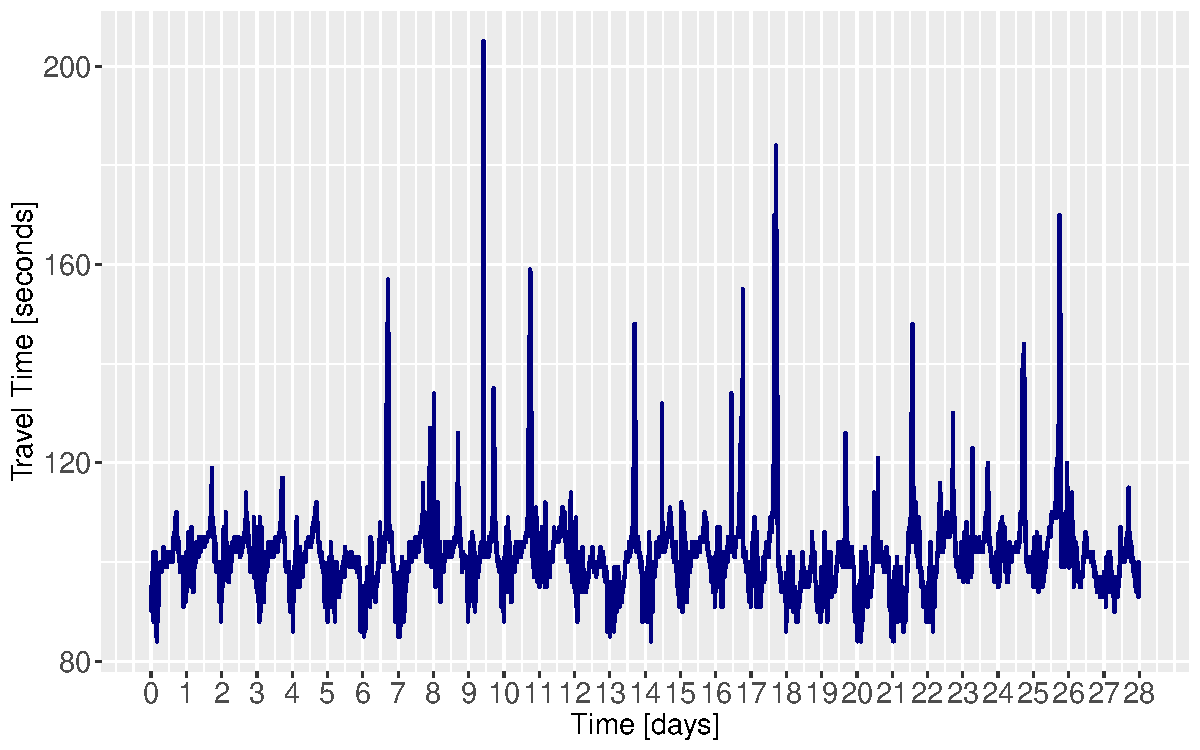
\includegraphics[width=\linewidth]{./images/Travel_Time.pdf}}
\caption{Travel time in link 1170079 of the M6 over a period of 28 days between 07/Mar/2016 and 04/Apr/2016.}
\label{fig:travel_time}
\end{figure}
In Figure \ref{fig:travel_time}, it can be observed that while most of the time, the travel time in a link repeats a vaguely predictable patterns during most of the days, with minima during nights corresponding with the bounded free flow time (except for speeding drivers).
As the morning rush starts, travel time will rise leading to the morning traffic jams which are generated from the collective drivers behaviour.
More effects of this collective dynamics can be observed in the afternoon during the evening rush; normally being able to find a plateau between these two peaks.
After this, the travel times progressively decay towards the night period of free-flow regime.
In Figure \ref{fig:travel_time}, we can also observe that there are a series of peaks found out of this oscillating yet typically bounded behaviour. 
In these, the travel time can increase up to several times fold the normal values.
These large oscillations are not nearly as predictable both in intensity and inter-oscillation period than the recurrent congestion described previously.
\begin{figure}[htbp]
	\centerline{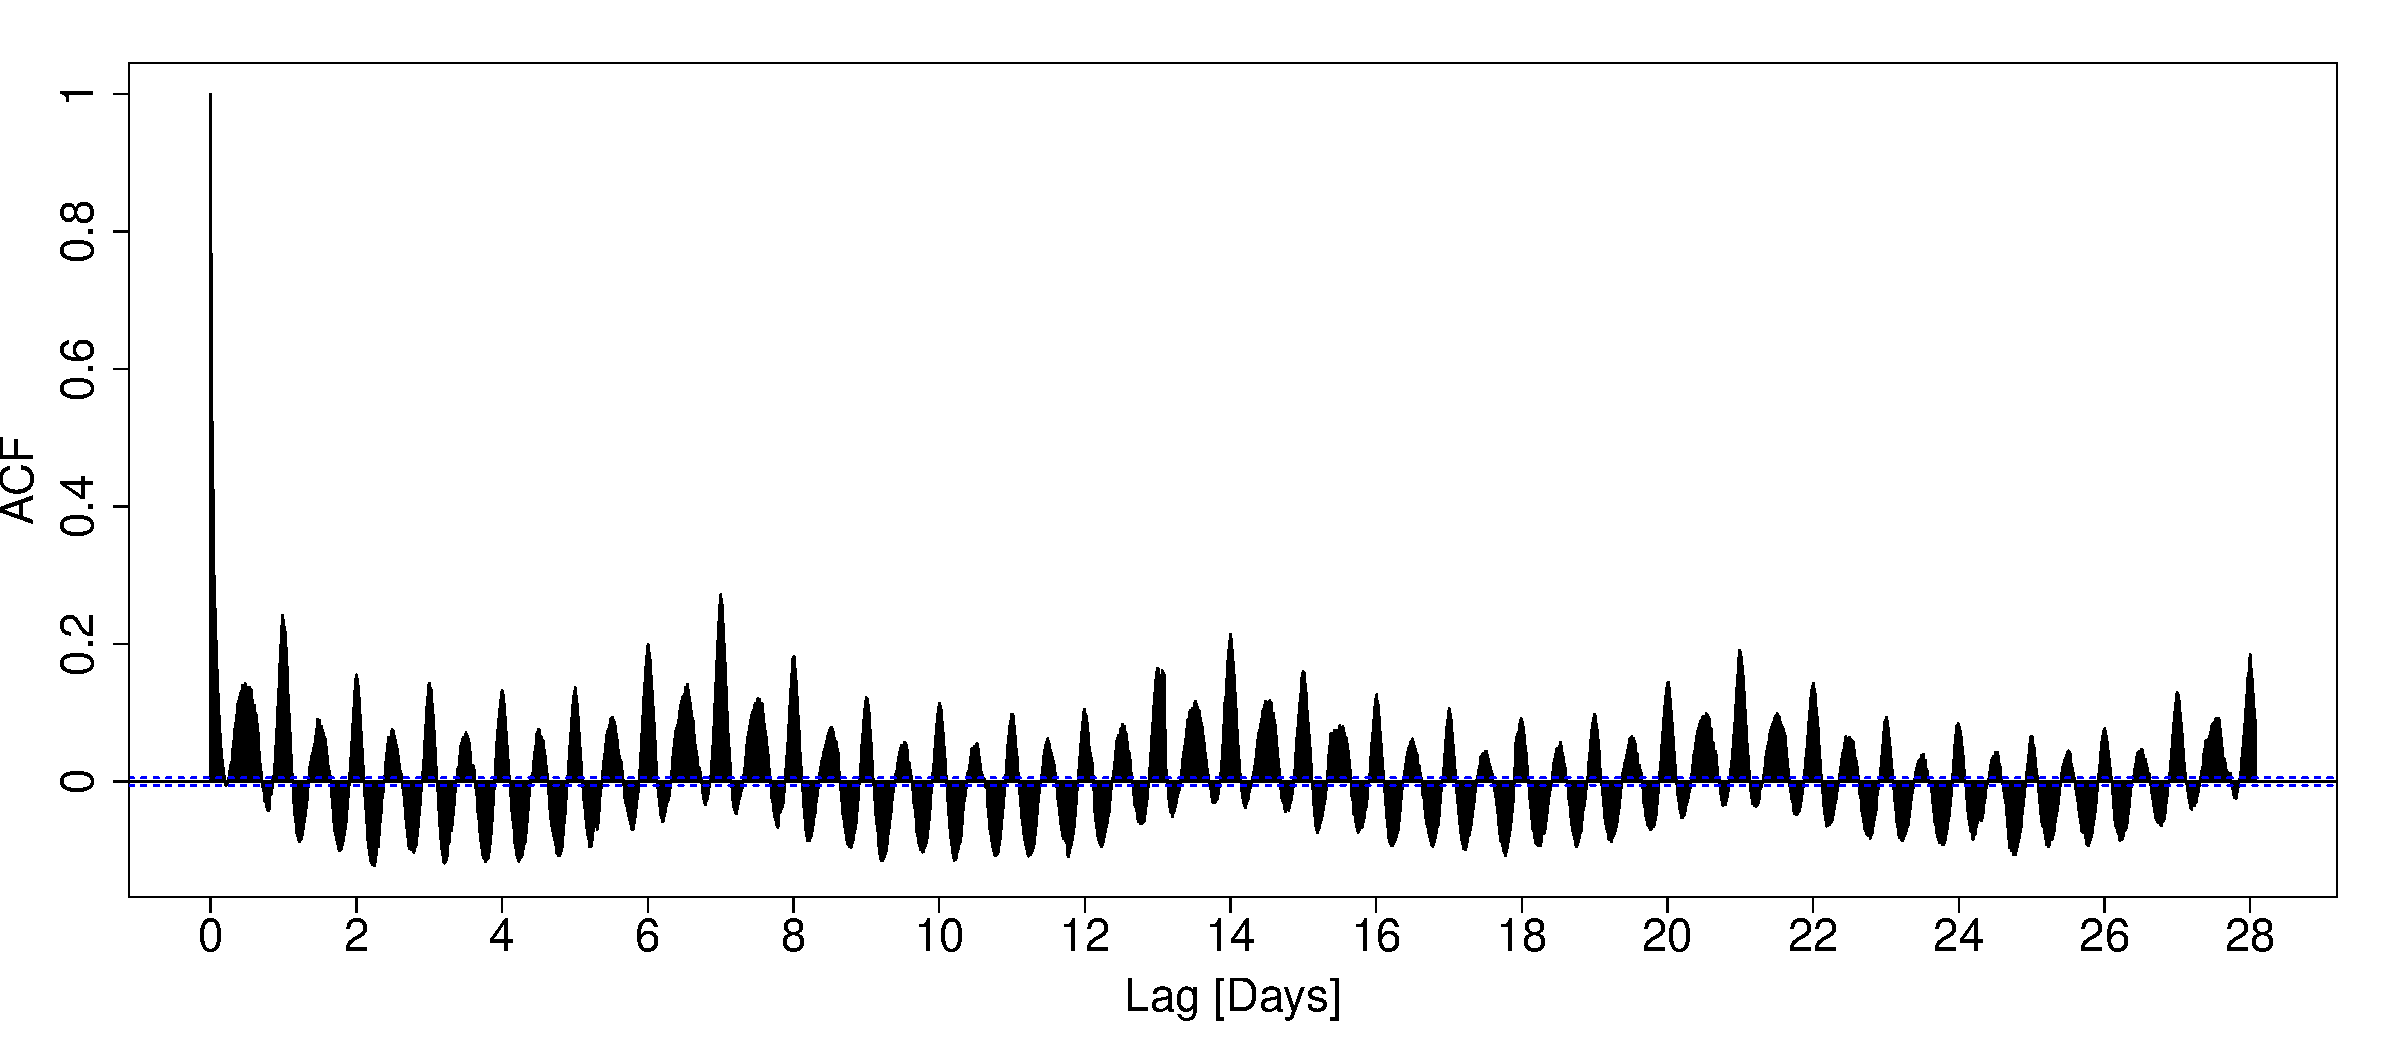
\includegraphics[width=\linewidth]{./images/ACF_M6_Link3.pdf}}
	\caption{Autocorrelation function of the Travel Time series in figure \ref{fig:travel_time} with a maximum lag of 4 weeks.}
	\label{fig:ACF}
\end{figure}
Lastly, in figure \ref{fig:ACF}, we can see the Autocorrelation Function for the Travel Time, plotted with a maximum lag of 4 weeks. Here we can see a double seasonal pattern with periods of 1 day and 1 week.
This regularity seen in time travel time series can and is often used by modellers to approximate and forecast travel times as is explored over the next sections.
\section{Basic methods for profile estimation}\label{Basic methods for profile estimation}
\subsection{Use of Exponentially Weighted Moving Average} \label{ewma}
As explained in \cite{ttprofiles}, the most basic approach to profile estimation is to apply an Exponentially Weighted Moving Average (EWMA) on the same minute of every day, assuming that similar behaviour is expected at the same time of the day. 
In this manner, the estimated profile $\hat{x}(i,d+1)$ on the $i-th$ minute of a given date $d$, for a memory parameter $\alpha \in [0,1]$ and with measured travel time $x_i^d$, will be:
\begin{equation}
\begin{aligned}
\hat{x}^{d+1}_i &= \alpha * x^{d}_{i} + (1-\alpha)*\hat{x}^{d}_{i} \\ 
&= \alpha * x^{d}_{i} + \alpha^2 * x^{d-1}_{i} + (1-\alpha - \alpha^2) \hat{x}^{d-1}_{i}\\ 
&= \alpha * x^{d}_{i} + \alpha^2 * x^{d-1}_{i} + \alpha^3 * x^{d-2}_{i} + \bigg( 1-\sum_{i=1}^{3} \alpha^i \bigg) \hat{x}^{d-1}_{i}\\
&= ...
\end{aligned}
\label{eq:ewma}
\end{equation}
The main issue with EWMA-based profiles is the effects generated due to the way in which the memory decays as we can see above in equation \ref{eq:ewma}.
\begin{figure}[htbp]
	\centerline{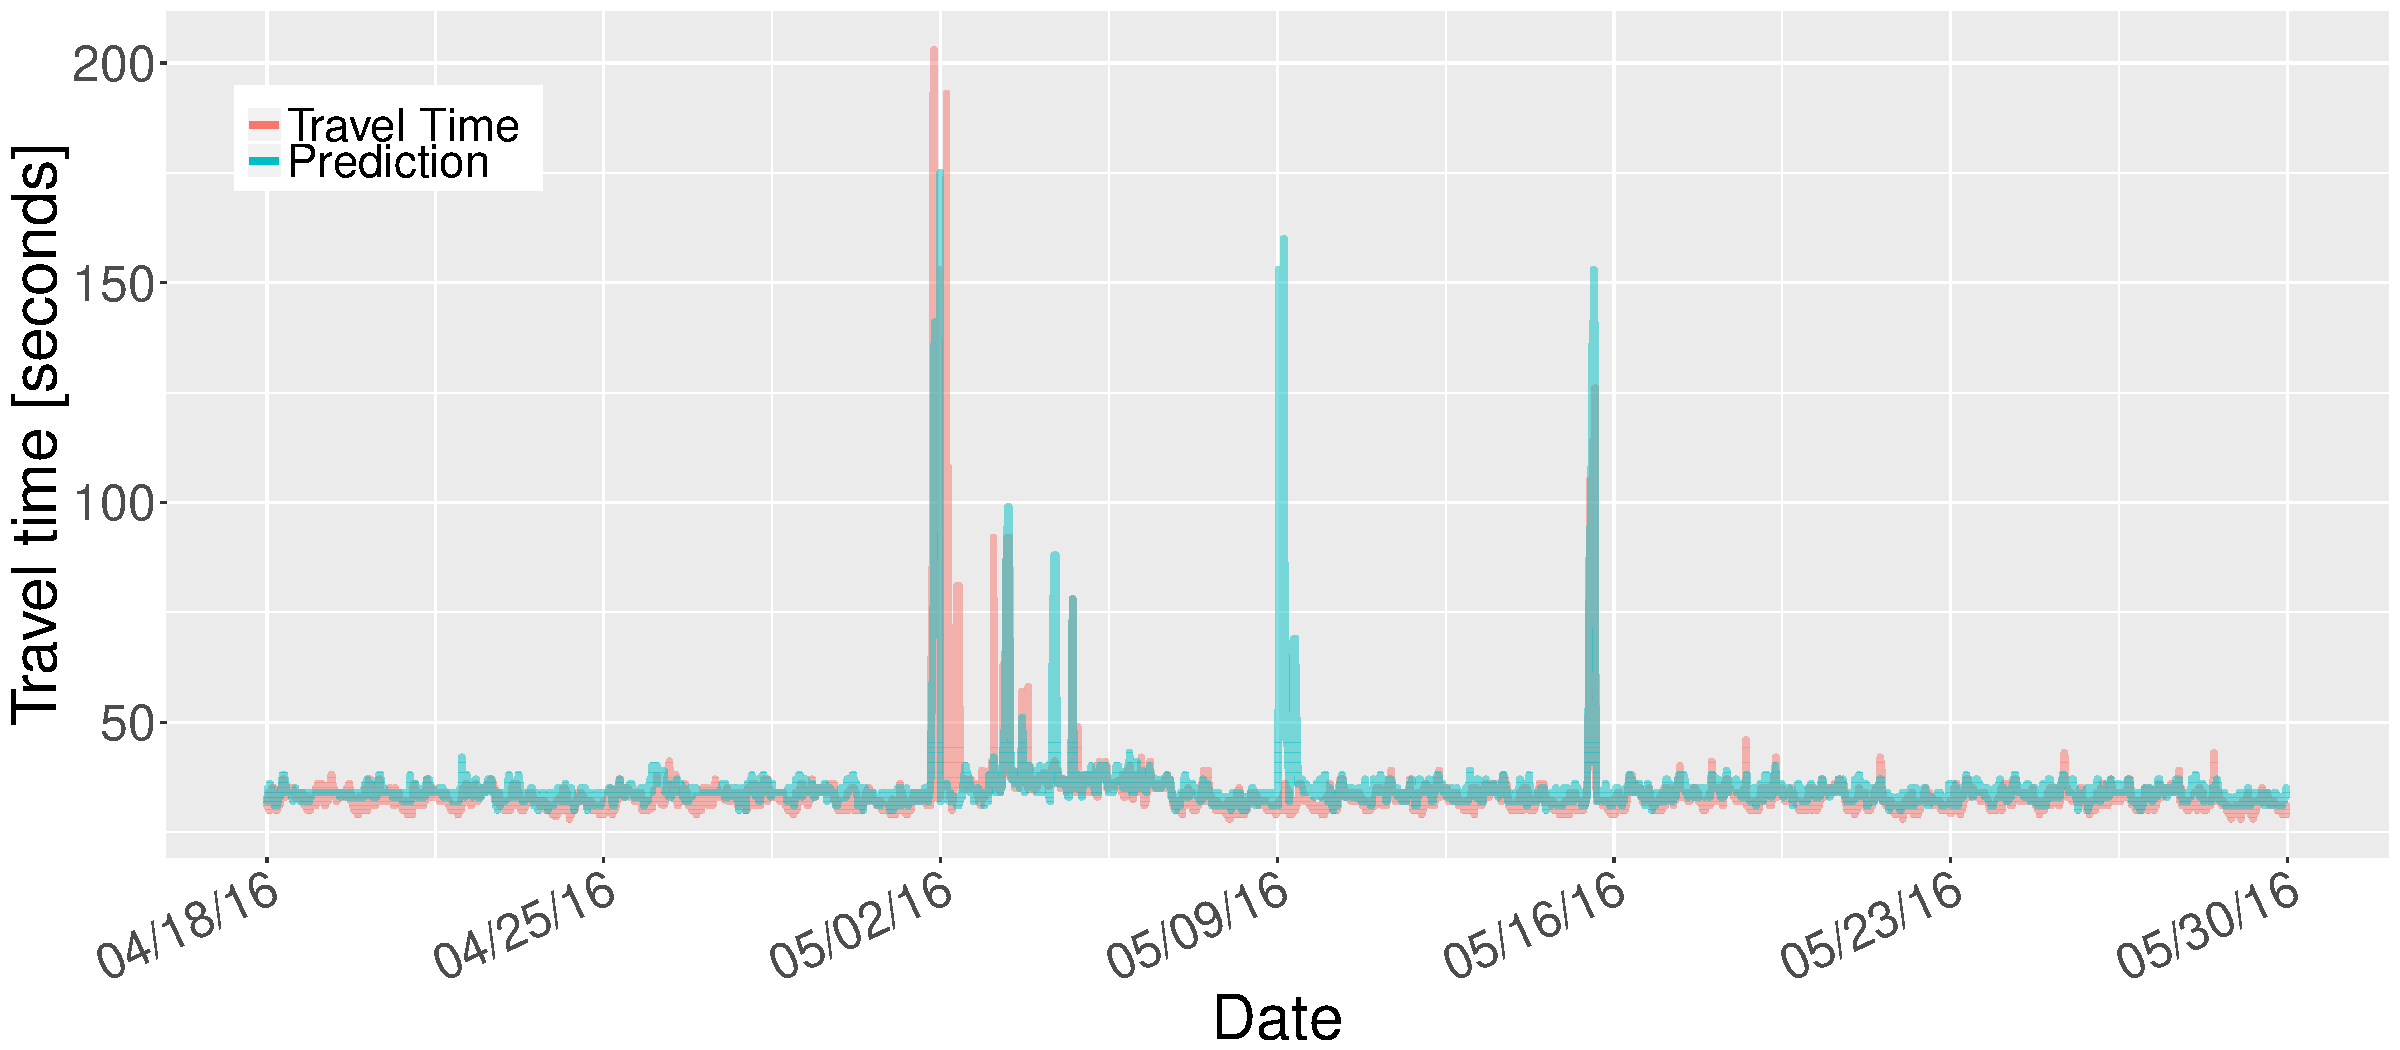
\includegraphics[width=\linewidth]{./images/EWMA.pdf}}
	\caption{False EWMA predictions after a large deviation.}
	\label{fig:EWMA}
\end{figure}
Recent measurements are weighted exponentially more heavily than events farther in the past. 
Thus if an extreme fluctuation occurs, the following profile estimates will be biased, partially replicating this event and over-estimating the travel times until enough new measurements arrive to dissipate this effect.
\subsection{Segmentation}\label{segmentation}
In addition, to recognize and use the specific differences of some special dates in the year, and the intra-week variation, this family of methods makes heavy use of date based segmentation. 
The EWMA is applied across dates which fall in the same category (i.e. Saturdays, weekdays, New Year, ...).
This segmentation in classes, when combined with the shortcomings presented in Section \ref{ewma} can generate some long lasting perturbations, which can propagate for weeks into the future predictions, while not being reflected on the observed travel times. A possible instance of this effect can be seen in Figure \ref{fig:EWMA}.
It follows that in order to generate a valid segmentation, operational and geographical expertise about specific roads is needed, given that the EWMA approach is effective exclusively for endemic congestion. 
This dependence can lead to the creation of legacy systems which become difficult to maintain after a few years, decreasing their usability over time unless extra effort is put into transmitting this knowledge and continually train new staff.
These modelling and staffing limitations make Segmentation and EWMA based profiles suboptimal both in performance and operation.
\section{Data}
\subsection{Data Gathering and Selection}
Data was gathered from 2 different Motorways in England.
The M6 and M11 were selected due to their high usage and combination of recurrent and outstanding congestion, being key in several heavily used commuting routes. 
\begin{itemize}
	\item The dataset comprises 90 days (12 complete weeks) of data (07/03/2016-05/06/2016).
	\item Links were discarded if they had more than 10\% of missing data or if they contained any access ramps.
	\item The previous condition left 14 different links in the M6 and 25 links in the case of the M11.
	\item Whenever missing data was detected for 10 or less minutes, it was linearly interpolated.
	\item Whenever missing data was detected for over 10 minutes, it was left as missing values.
\end{itemize}
The initial 8 weeks are used by the algorithm to predict one complete week ahead.
One week later, the process is repeated, deleting the oldest week of training data and incorporating measurements of the week predicted in the previous step. 
This procedure is performed 4 times.
\subsection{Data Contents}
For each link on a specific date, the data consists of one sample per minute, containing:
\begin{itemize}
	\item Measured travel time
	\item Profile (expected) travel time 
	\item Traffic Flow
	\item Overhead Space	
\end{itemize}

\section{Background and Spikes}
\subsection{Characteristics}
As described in \cite{ttprofiles}, during our initial exploration of the data we found that, from the point of view of travel times, traffic operates in two differentiated regimes that we denominated Background and Spikes. 
\begin{itemize}
	\item Background: 
	\begin{itemize}
		\item Stable around a mean value.
		\item Oscillates with small amplitude and high frequency.
		\item Suitable for spectral filtering (smoothing) and seasonal analysis.
	\end{itemize}
	\item Spikes: 
	\begin{itemize}
		\item Zero most of the time.
		\item Quickly go to extreme values.
		\item Oscillates with great amplitude and high inter-oscillation period, creating far reaching effects.
		\item Non-periodic as per detection in time-frequency domain, however, non harmonic seasonality can be extracted via non-parametric regression .
	\end{itemize}
\end{itemize}

In this context, if we assume Gaussian noise $\xi$, and that the Background and Spike components will operate in an additive way, the decomposition will be of the form:
\begin{equation}
\textrm{Travel Time}_t  = \textrm{Background}_t + \textrm{Spikes}_t + \xi
\end{equation}
The objective is to separate them in such a way that the moments of smooth and normal operation, together with the recurring congestion are captured as part of the Background and used for spectral smoothing, attempting to mitigate the prediction error induced by the high frequency oscillations and obtaining a basic view of what can be daily observed, so seasonal patterns can be extracted in the shorter and longer periods shown in \ref{fig:ACF}.
Meanwhile, the spikes, containing the non-recurring congestion, can be treated separately searching for seasonality left in larger time scales than those in which the travel time signal oscillates, as also suggested by Fig. \ref{fig:ACF}. 
Ideally, after this seasonal extraction step of the decomposition, the remainder should only contain isolated large rare events deviating from the profile and white noise.
\subsection{Wavelet Time Series Decomposition}\label{decomposition}
\begin{figure*}[htbp]
	\centerline{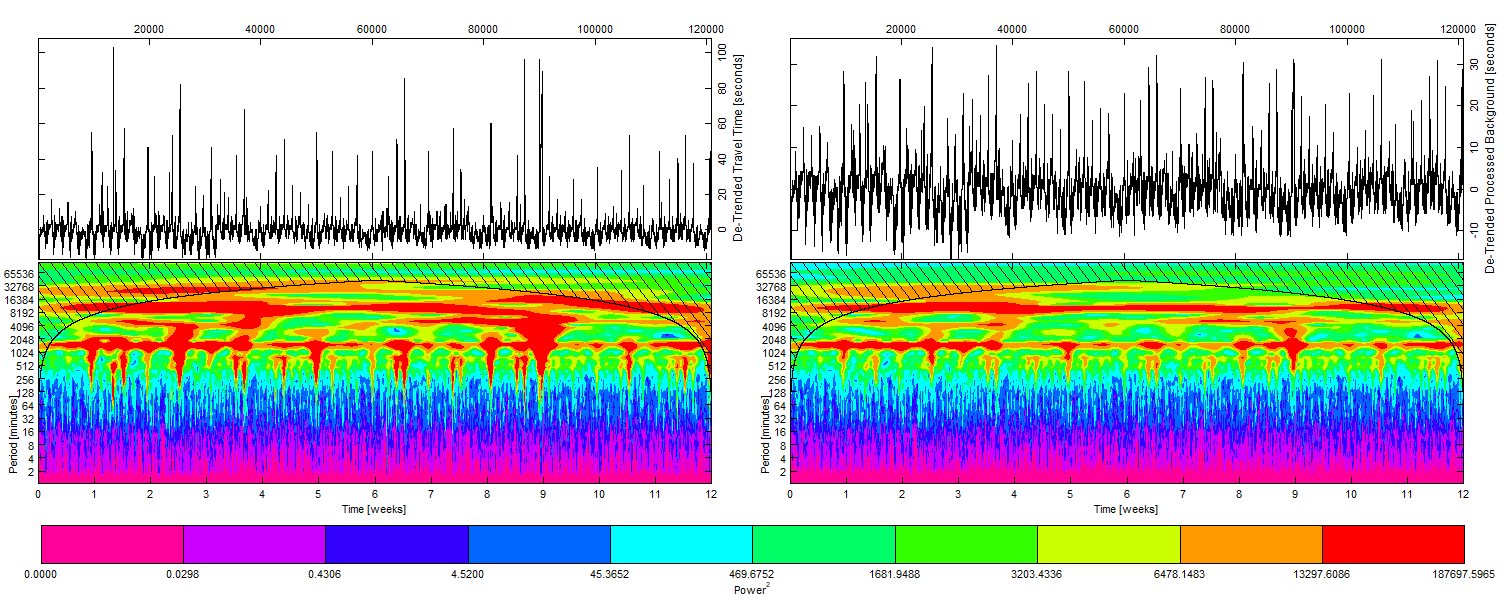
\includegraphics[width=\linewidth]{./images/WT_combined_1500_600.png}}
	\caption{Left: Power of DWT of the original Travel Time series for Link 1170079 of the M6.
	Right: Power of DWT of the extracted Background $\vec{B_t}$ series, as detailed in Section \ref{decomposition}, for Link 1170079 of the M6}
	\label{fig:wt}
\end{figure*}

To perform the decomposition, we will take advantage of the additive properties of the wavelet transform. First the time series $\vec{x_t}$ of length $t$, and elements $x_i$ with $i in [0,t]$ is turned into a zero mean series $\vec{x_t} - mean(\vec{x_t})$ and used as input for a Continuous Wavelet Transform (CWT) \cite{daubechies} \cite{mallat} using a Morse wavelet \cite{morse} and 140 timescales levels.
The output of this first transform is a complex matrix $\vec{W}_{\textrm{levels}\,\times\, t}$, for the elements of which we calculate their modulus $\rho$, phase $\phi$ and power $P$. 
A heatmap of $P^2$ for the original time series can be seen in the first subplot in Figure \ref{fig:wt}.
In the figure we can observe that the most influential dynamics occurring during the series length, happen at the timescales where it was expected based on Figure \ref{fig:ACF}, namely 1 day (1440 minutes) and 1 week (10080 minutes).
In the figure, we also observe that surges in power across different timescales occur at the same time as the non-recurring congestion, since in order to approximate this signal, the CWT algorithm needs to combine several wavelets with smaller periods than those dominating the recurring part of the series.

In order to isolate this non-recurring component, the series is sequentially assessed over all the time domain for a single timescale level $l$, generating a series $\vec{x_{t}}^l$.
After fixing $l$, we calculate the Median and Inter Quantile Range of $\vec{x_{t}}^l$ to search for outliers.
A maximum threshold value is set equal to $T = median(\vec{x_t}) + \alpha * IQR(\vec{x_{t}}^l)$, with $\alpha \in [0,\inf]$ being a parameter that defines how aggressively we target spikes. 
The results produced here were obtained with $\alpha=1$ to showcase the most basic setup.

Then, the individual elements of $\vec{x_{t}}^l$, $x_{i}^l$ are individually evaluated: if found below the limit, they are stored in a Background container $B_i^l = x_{i}^l$; otherwise, the fraction below the threshold will be nonetheless passed on to the background $\vec{B_i}^l = median(\vec{x_{t}}^l) + \alpha * IQR(\vec{x_{t}}^l)$, with the remaining part going into the Spikes storage $\vec{S_i}^l = x_{i}^l - B_{i}^l$.

Once all levels have been processed in this manner, we use the previous information about $\phi$ to reconvert the two series from being characterised in terms of $(\rho, \phi)$ to the complex components of the DWT.
After this step, we apply the Inverse DWT to $\vec{B_t}$ and $\vec{S_t}$, obtaining the two series that can be observed in Figure \ref{fig:splitting}.
\subsection{Series Recombination}
\begin{figure}[htbp]
	\centerline{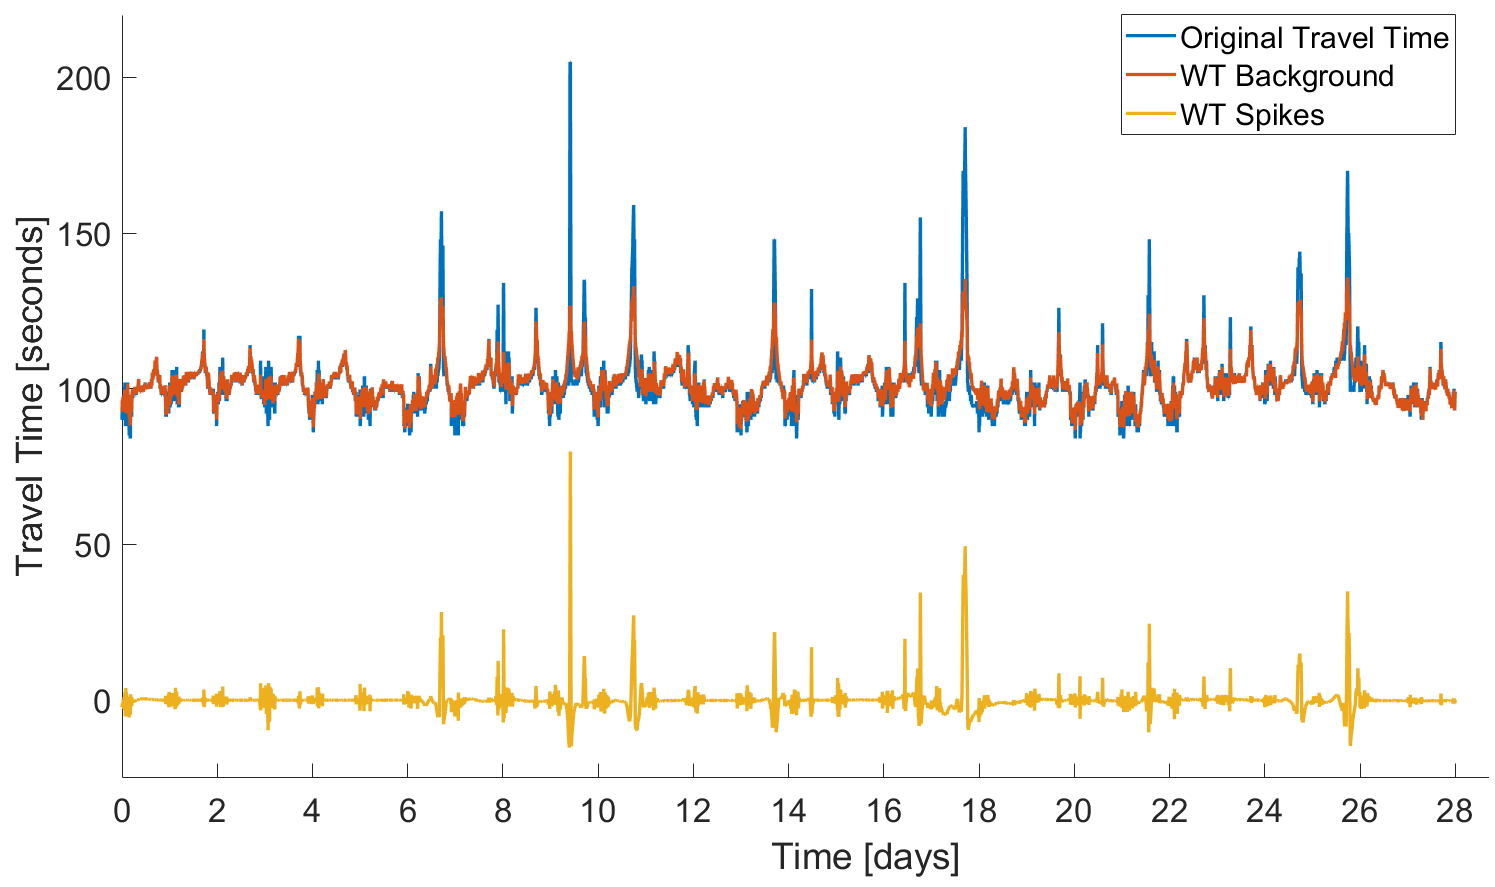
\includegraphics[width=\linewidth]{./images/Splitting.png}}
	\caption{Recombination}
	\label{fig:splitting}
\end{figure}

Due to small noise introduction during the inverse transform a threshold is applied to $\vec{S_t}$, where elements representing spikes of less than 3 seconds in amplitude are set to zero.

For future prediction steps, an indicator function was defined, taking for every minute the value:
\begin{equation}
    \delta_i^{spike}=
    \begin{cases}
      1, & \text{if } x_i > \text{Threshold}\\
      0, & \text{otherwise.}
    \end{cases}
    \label{delta}
  \end{equation}
  


\section{WARWICK Travel Time Prediction Algorithm} \label{algorithm}
Given the cyclic nature of traffic, the aim was a prediction algorithm that could account for the periodic variations and endemic congestion while being resilient to fluctuations and rare events. This algorithm also should:
\begin{itemize}
	\item Be robust, mitigating the propagation of isolated events into future forecasts, unlike methods using EWMA.
	\item Not require the use of time segmentation and be valid for regular and "special" dates.
	\item Be location agnostic, the internal parameters should be set algorithmically based on the data.
	\item Have Gaussian, mean 0, uncorrelated residuals.
	\item Near flat Trend term, given the different time scales between seasonal cycles and changes in the general motorway flow.
\end{itemize}

\subsection{Naive Segmentation (Null)}
To obtain an accurate comparison of the performance of the algorithm developed in the following subsections, an example of basic segmentation was coded. 
This involved a weighted combination of the training data points using uniform weights. 
In this way, for the $i-th$ minute of a week and using a training set composed of the previous of $n$ weeks, the Naive Segmentation (NS) profile is:
\begin{equation}
\hat{x}(i,n) = \sum_{\textrm{week}=1}^{n} \frac{x^i_n}{n} 
\end{equation}

\subsection{WARWICK: Spectral Component}
The main difficulty when dealing with the Background signal is the low amplitude, high frequency fluctuations that can be found almost ubiquitously. 
Signal smoothing can be performed by completely removing a range of frequencies while the information bearing bands are retained. For this task, the Fast Fourier Transform (FFT) \cite{FFT} was used as follows:
\begin{enumerate}

	\item Calculate Background Power Spectrum using FFT
	\item Remove frequencies corresponding to periods under 4 hours and over 1 week
	\item Repeat for all $n$ weeks in training set
    \item Apply EWMA to the modified weekly Power Spectra
	\item Compute the Inverse FFT Transform

\end{enumerate}
\subsection{WARWICK: Seasonality Component}
Seasonal-Trend Decomposition based on LOESS (STL) \cite{STL} was the chosen algorithm for the seasonality analysis since it can handle any type of seasonality, allowing the user to control how it changes over time as well as the smoothness of the trend-cycle while being highly robust to outliers \cite{forecasting}.\\

Below, the sequence of steps taken to extract the Seasonality Components that can be observed in Fig. \ref{fig:ACF} is described in line with the schematic data streams represented in Fig. \ref{fig:flowchart}. 
Note that this should be applied to the $n$ training weeks as a single time series.
\begin{enumerate}
	\item Decomposition of Background for daily seasonality
	\item Extract and sum the series corresponding Trend and Remainder from Step 1
	\item Decomposition of output from 2 for weekly seasonality
	\item Add daily and weekly Seasonal components from Step 1 and Step 3 to obtain global seasonality
	\item Average seasonality across training weeks
	\item Linearise Trend term from output of Step 3
	\item Add linearised trend to seasonality obtained in Step 6
	\item STL Decomposition of Spikes for weekly seasonality
	\item Extract Spike's Seasonality corresponding to the number of weeks for forecasting
	\item Add Spike's Seasonal component to the output of 8
\end{enumerate}
To ensure a successful decomposition, after performing Step 3, the Background's Remainder should be zero mean, Gaussian distributed. Background's Trend should have a near zero slope. These outcomes should also hold if performed again after Step 8, with the addition that the trend should also be close to zero in absolute value, since the time scales in which such a global trend can meaningfully vary should be much greater than the prediction scope of this algorithm.
\subsection{WARWICK Hybrid Profile}
In order to create the final Seasonal-Spectral Hybrid profile (Hybrid), one of the two forecasts generated in the previous points is taken, depending on what is the identified regime: 

\begin{equation}
\textrm{Hybrid} = \textrm{Seasonal} * \delta_{\textrm{spike}} + \textrm{Spectral} * (1 - \delta_{\textrm{spike}})
\end{equation}


\begin{figure}[htbp]
	\centerline{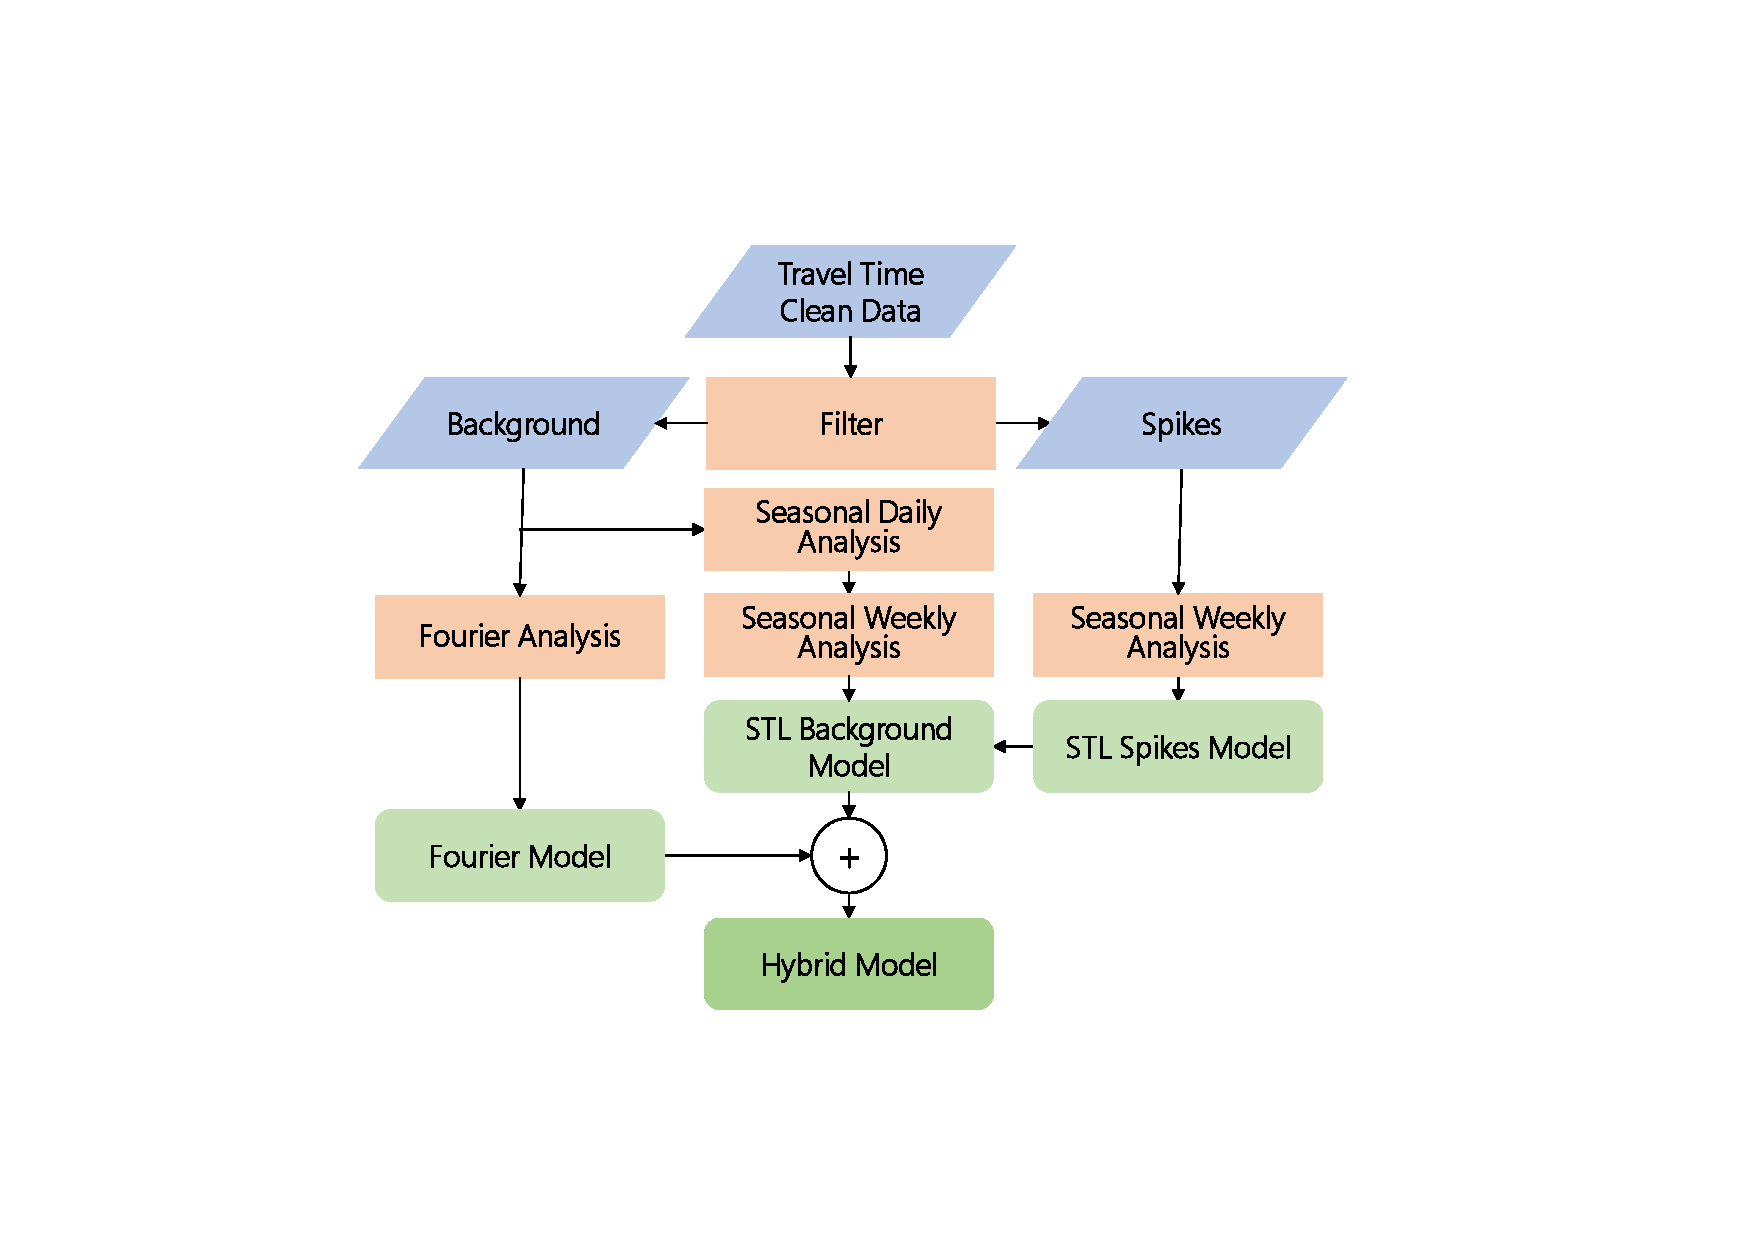
\includegraphics[width=\linewidth]{./images/flow_temp.pdf}}
	\caption{Things}
	\label{fig:dataflow}
\end{figure}



\section{Accuracy Results}
\begin{table*}[bp]
	\caption{WARWICK Profile - MARE Distribution Per Motorway}
	\centering
	\begin{center}	
		\begin{tabular}{|C|C|C|C|C|C|C|C|C|}
			\hline
			\textbf{\% rel. error}&{\textless -25\%}&{-25\%\textbf{ to }-15\%}&{-15\%\textbf{ to }-5\%}&{-5\%\textbf{ to }5\%}&{5\%\textbf{ to }15\%}&{15 \%\textbf{ to }25\%}&{\textgreater 25\%}\\
			\hline
			M6& 1.57& 0.51& 3.22& 81.73& 12.14& 0.70& 0.13\\
			\hline
			M11& 0.78& 0.32& 3.29& 81.33& 12.47& 1.09& 0.73\\
			\hline
		\end{tabular}
		\label{mapeglobal}
	\end{center}
\end{table*}

\begin{table*}[bp]
	\caption{Publised Profile - MARE Distribution Per Motorway}
	\centering
	\begin{center}
		\begin{tabular}{|C|C|C|C|C|C|C|C|C|}
			\hline
			\textbf{\% rel. error}&{\textless -25\%}&{-25\%\textbf{ to }-15\%}&{-15\%\textbf{ to }-5\%}&{-5\%\textbf{ to }5\%}&{5\%\textbf{ to }15\%}&{15 \%\textbf{ to }25\%}&{\textgreater 25\%}\\
			\hline
			M6& 1.58& 0.54& 5.69& 56.21& 30.79& 3.17& 2.02\\
			\hline
			M11& 0.85& 1.15& 19.21& 62.83& 13.21& 1.65& 1.10\\
			\hline
		\end{tabular}
		\label{mapeglobal}
	\end{center}
\end{table*}
In this section the accuracy of the algorithm described above is compared against the Published Profiles and the NS Model. 
For each temporal point $i$, with a prediction $\hat{x_i}$, and an actual value of $x_i$, the Mean Average Relative Error (MARE) is defined below as:
\begin{equation}
\textrm{MARE} =\frac{ \left( \sum_{i=1}^{n} \frac{\|x_i - \hat{x_i}\|}{x_i}\right)}{n}
\end{equation}
For complete Motorways, the Root Mean Squared Error (RMSE) has been calculated for each temporal point $i$ as:
\begin{equation}
\textrm{RMSE} = \sqrt{\frac{\sum_{i=1}^{n} (x_i - \hat{x_i})^2}{n}}
\end{equation}
In both cases the error for a Link is defined as the average MARE or RMSE across all prediction points.
The error for a Motorway is defined as the average of the error across all its links.
\begin{figure}[htbp]
	\centerline{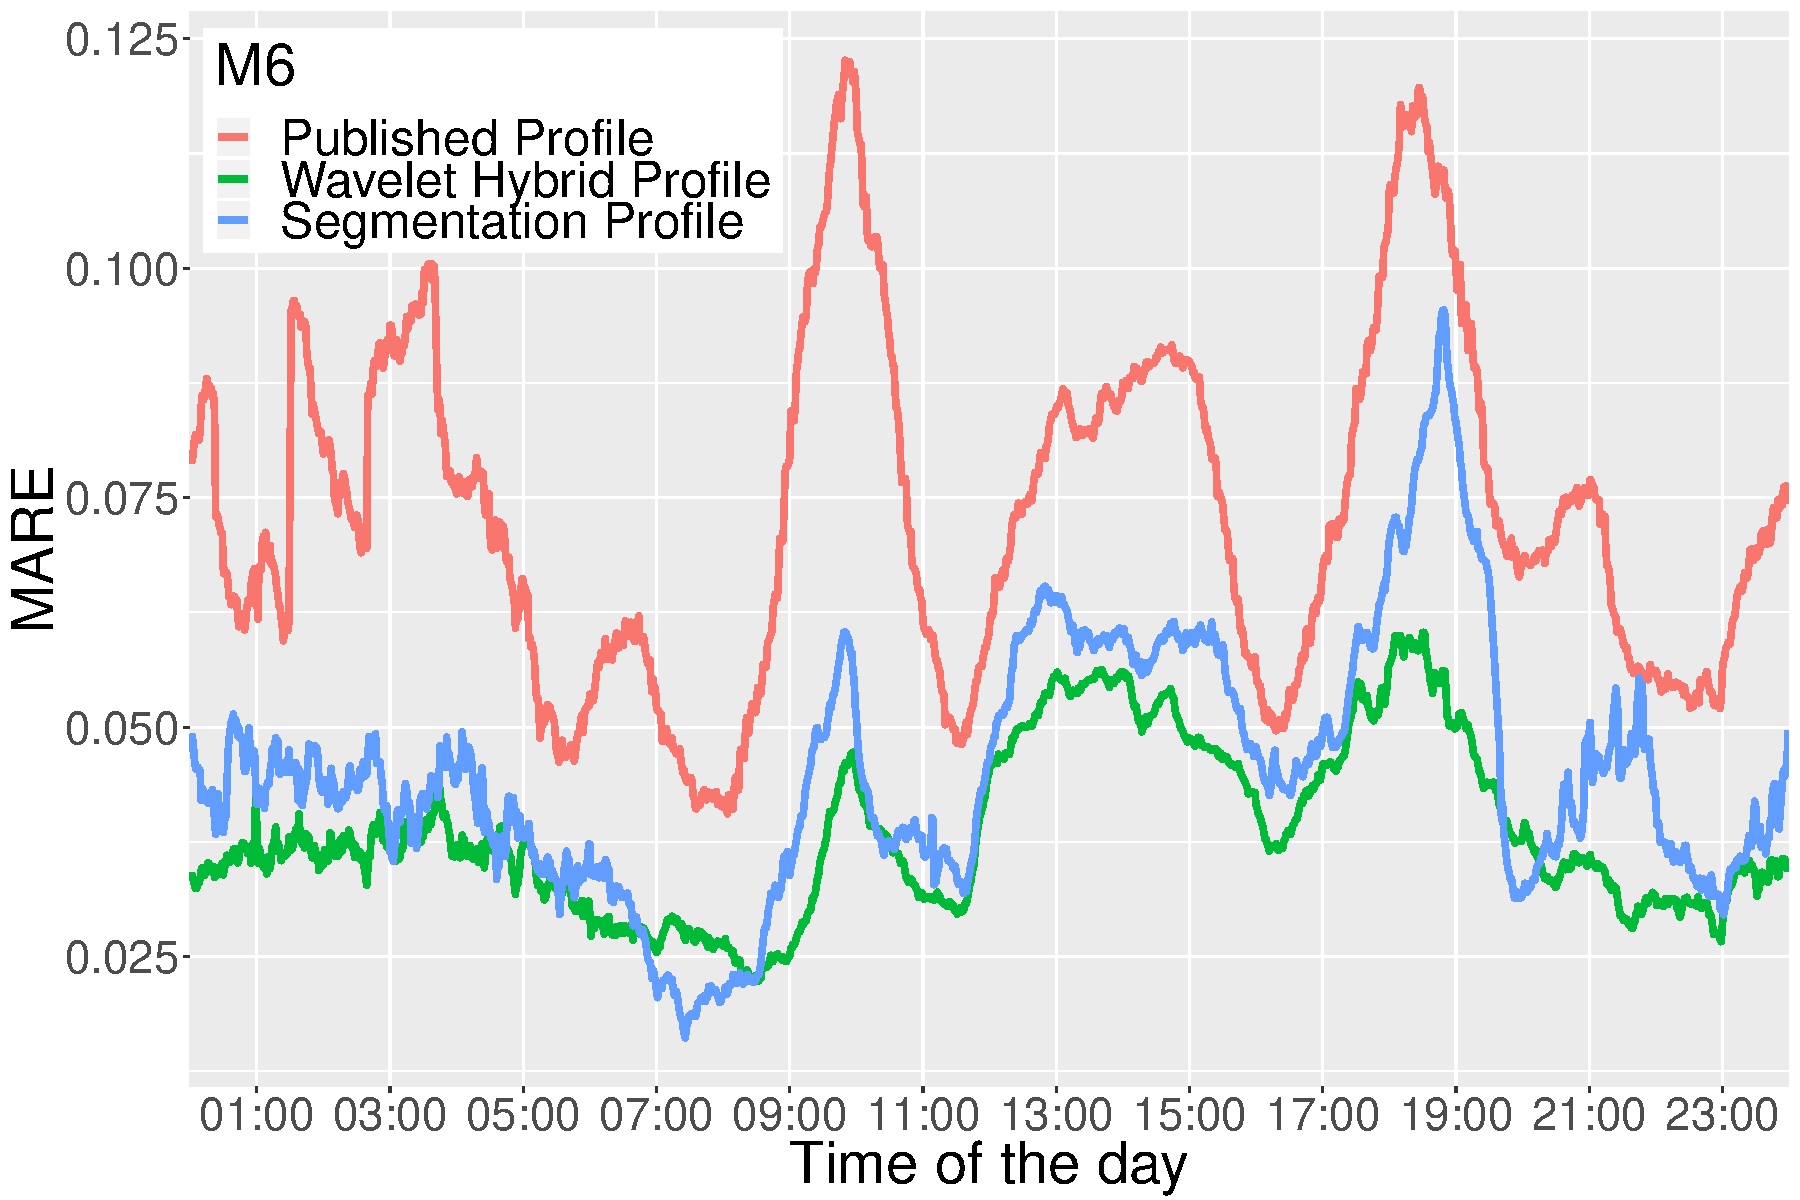
\includegraphics[width=\linewidth]{./images/M6_daytime_8_12.pdf}}
	\caption{MARE over the times of the day for the M6}
	\label{fig:m6dt}
\end{figure}
\begin{figure}[htbp]
	\centerline{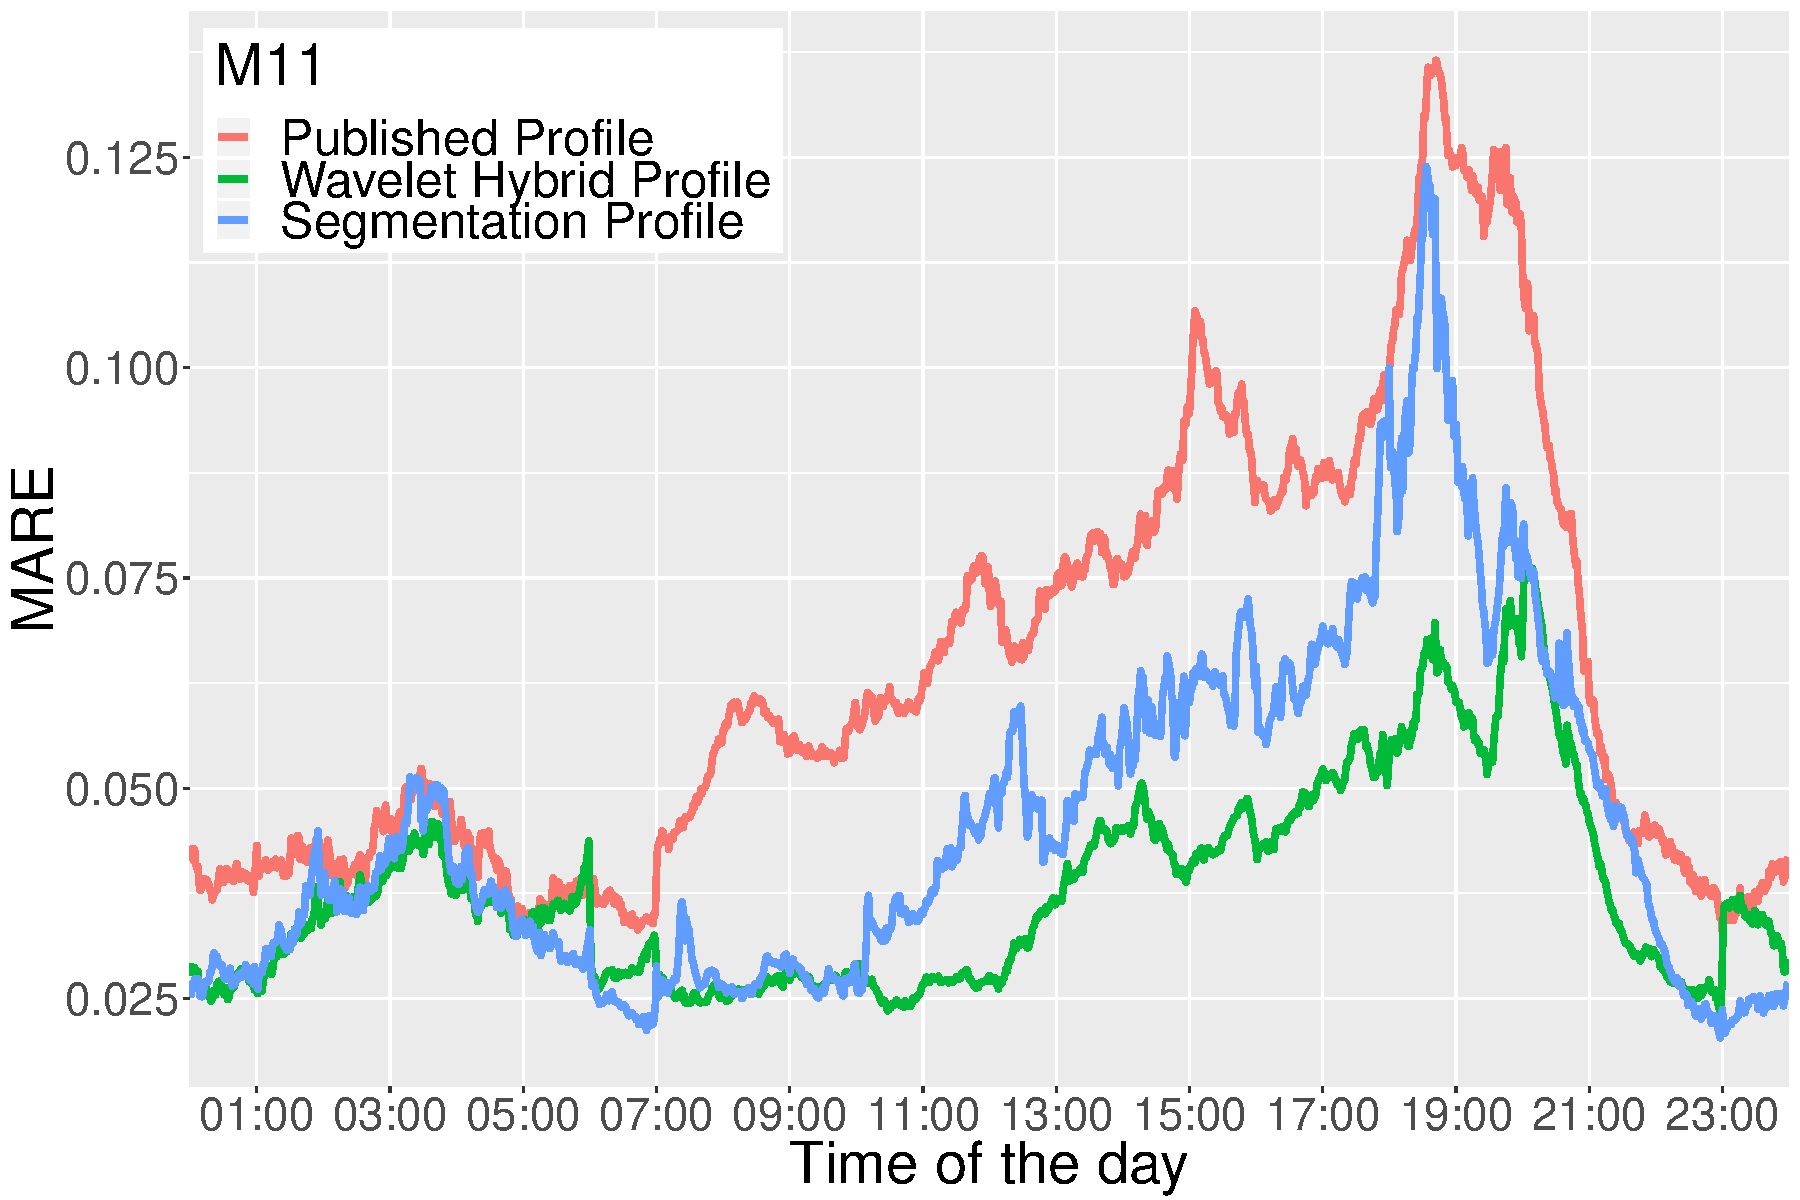
\includegraphics[width=\linewidth]{./images/M11_daytime_8_12.pdf}}
	\caption{MARE over the times of the day for the M11}
	\label{fig:m11dt}
\end{figure}


Here, the accuracy of the algorithm is compared against the Published Profiles and the NS Profile across all percentiles of travel time.
As it can be seen in Figs. \ref{fig:m6q} and \ref{fig:m11q}, the WARWICK Profile has a higher accuracy than the Published Profiles and the NS Model for all percentiles of travel time except for the most extreme values where they all perform poorly.\\
The most meaningful difference occurs between percentiles $[50-95]$, where the Published Profile starts to suffer from higher inaccuracy.

\begin{figure}[htbp]
	\centerline{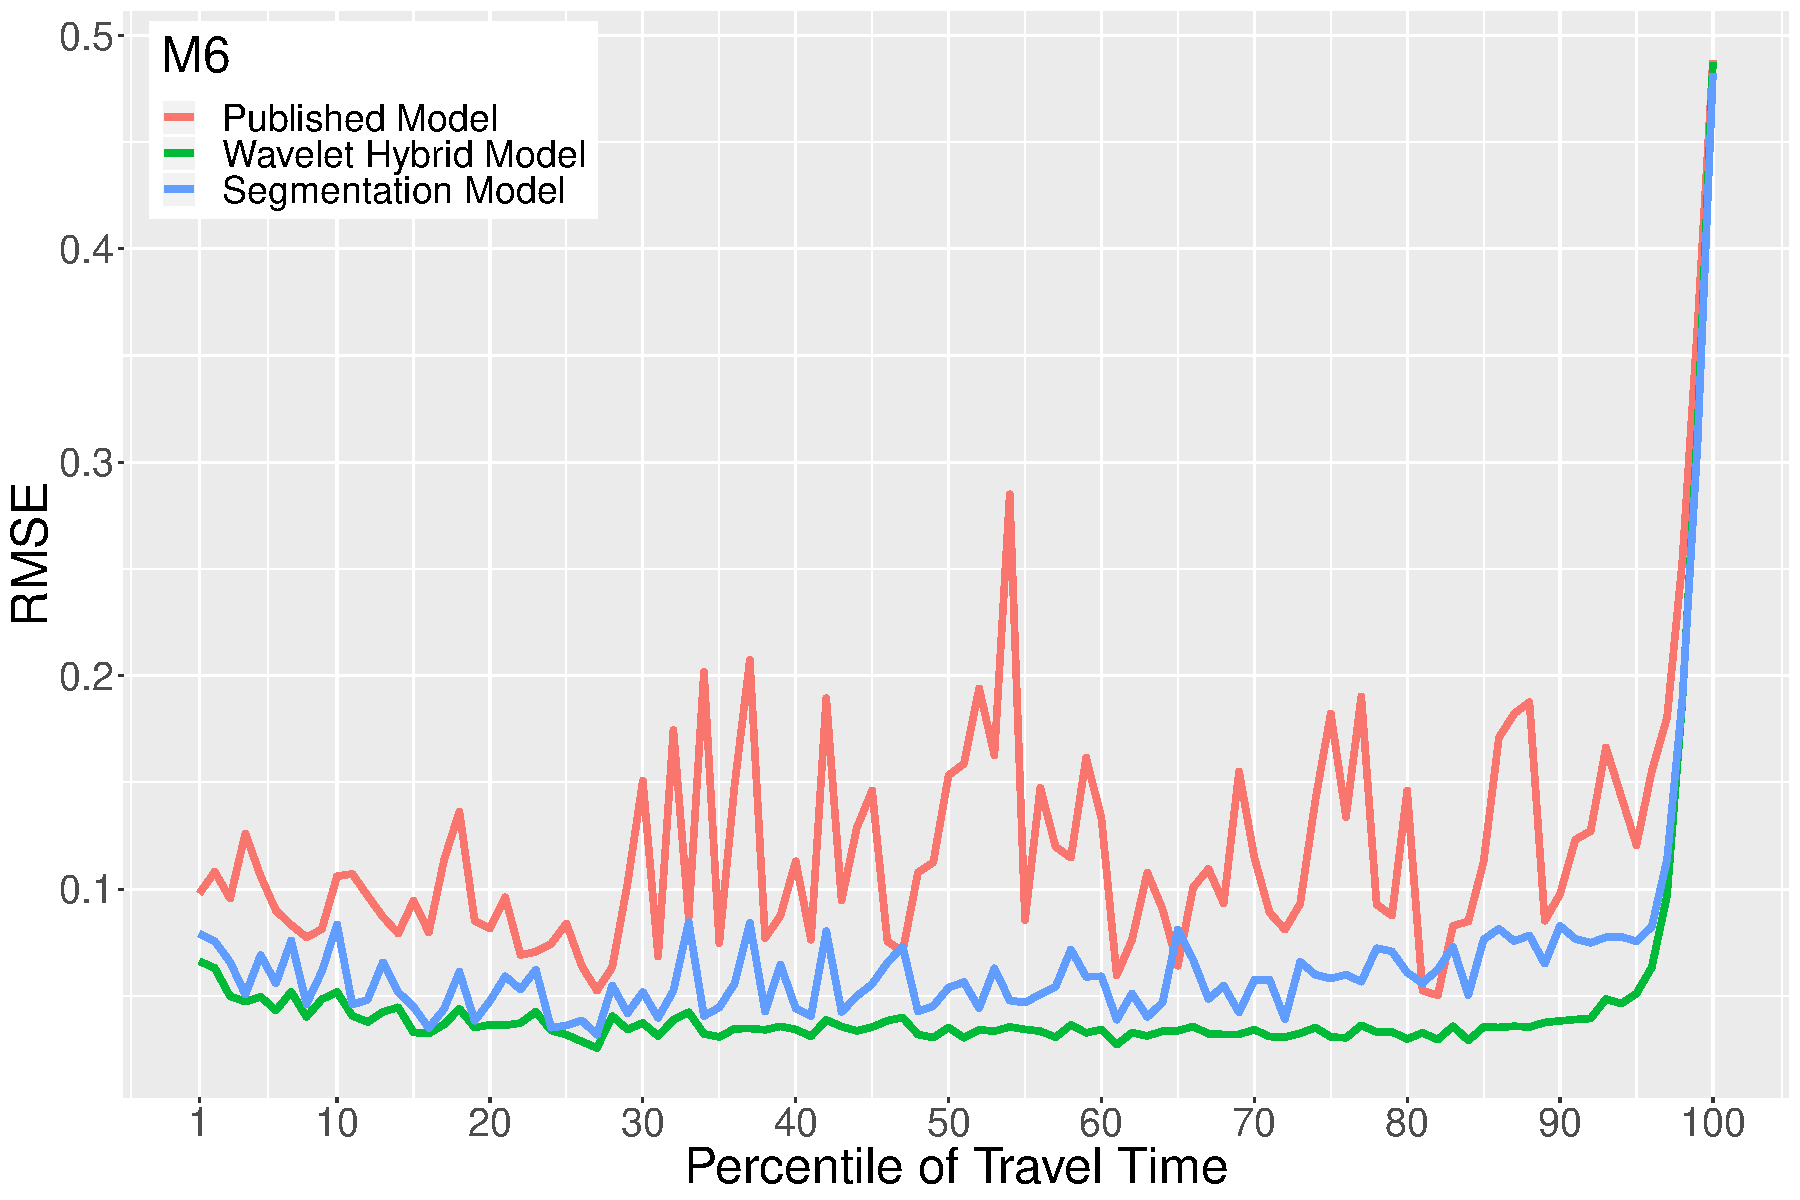
\includegraphics[width=\linewidth]{./images/M6_quantile_1_rms_8_12.pdf}}
	\caption{MARE across percentiles of travel time for the M6.}
	\label{fig:m6q}
\end{figure}
\begin{figure}[htbp]
	\centerline{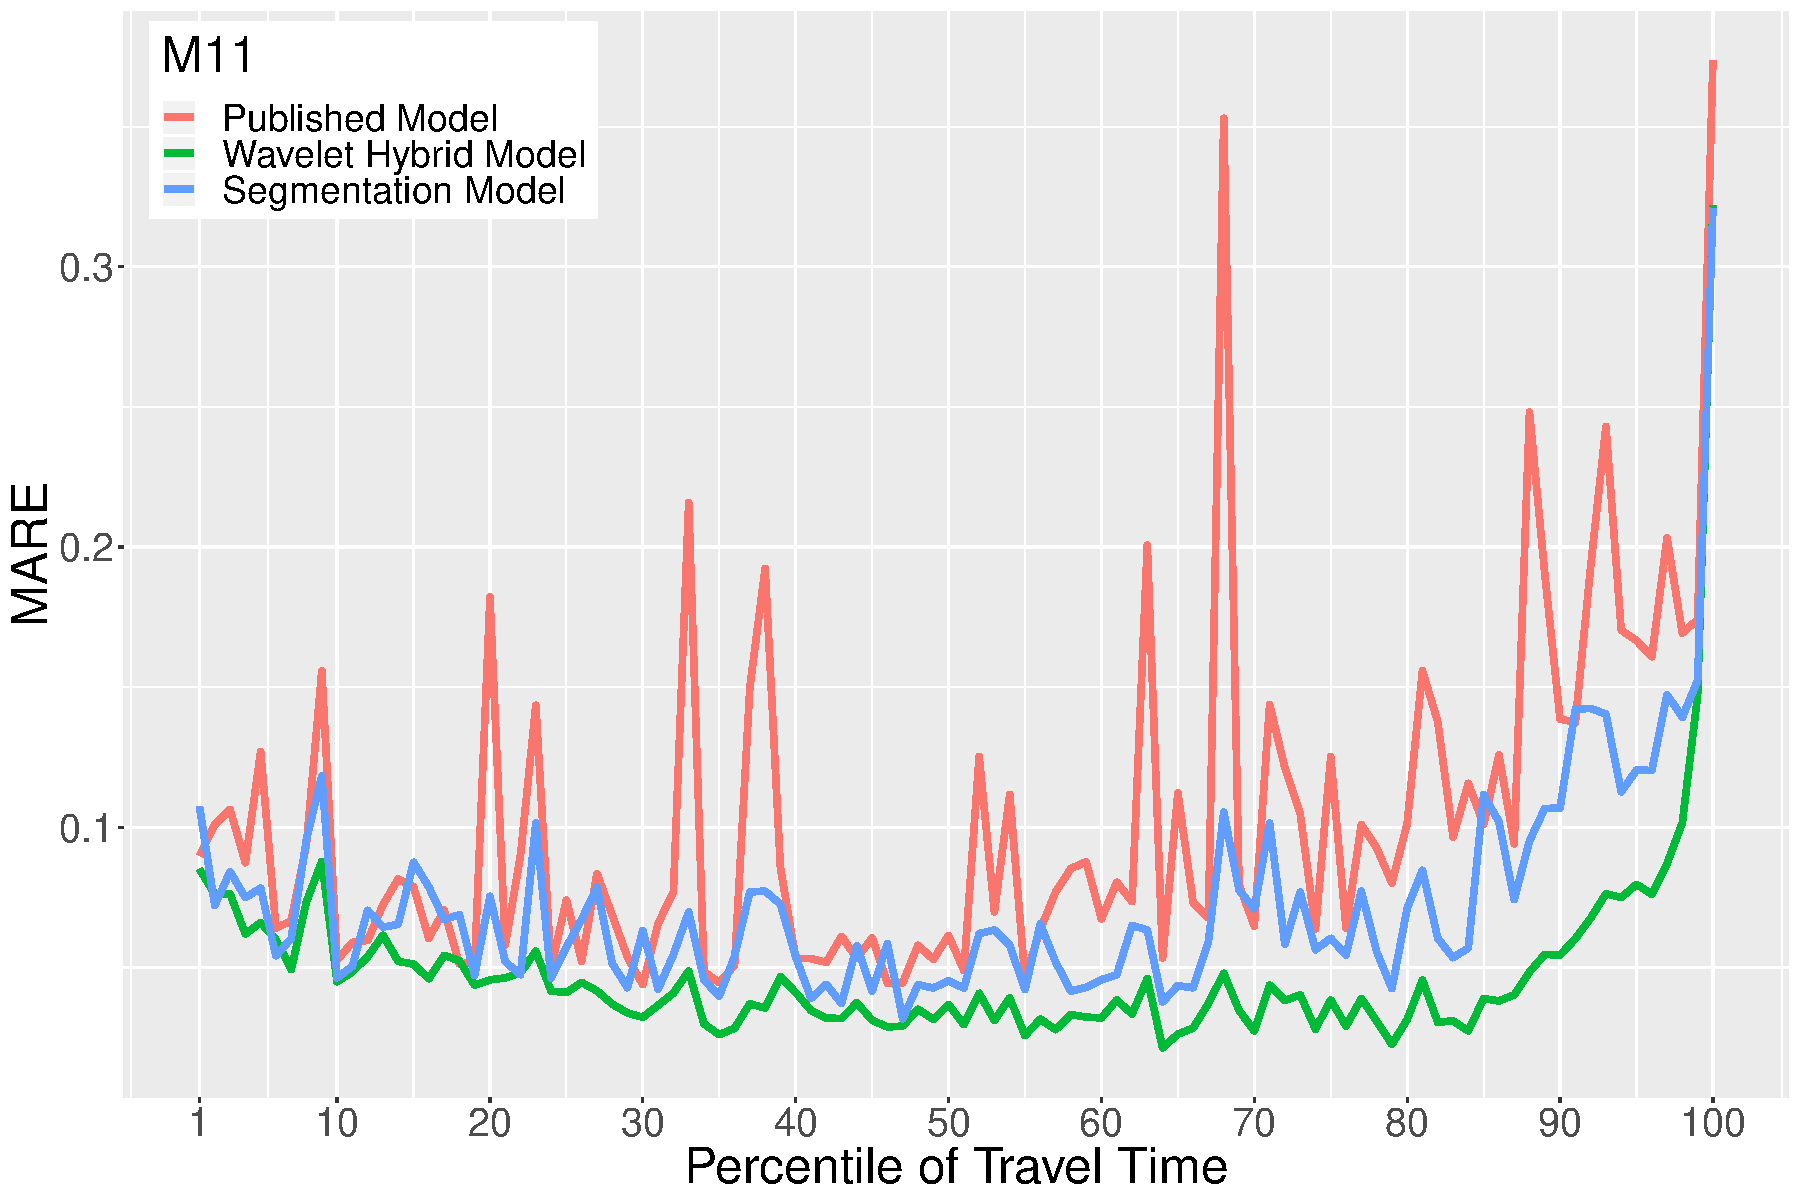
\includegraphics[width=\linewidth]{./images/M11_quantile_1_rms_8_12.pdf}}
	\caption{MARE across percentiles of travel time for the M11.}
	\label{fig:m11q}
\end{figure}

Here, the accuracy of the algorithm is compared against the Published Profiles and the NS Profile across the times of the day.
As it can be seen in Figures \ref{fig:m6dt} and \ref{fig:m11dt}, the Hybrid Profile has a higher accuracy than the Published Profiles and the NS Model for all times of the day, all locations and training lengths. 
The most relevant improvement occurs during the morning and evening peak hours, where the algorithm presented in this paper does not accuse meaningful performance worsening relative to the morning plateau when compared with the other two profiles.\\
In the case of the M6 and M11, where the training set is richer, the error at peak times is reduced by at least 50\% in all cases, reaching as much as 68.7\% in the case of the M6 morning rush.
In the case of the M25, which is congested on a regular basis, the errors in the Published Profile during peak times are slightly lower than on the other cases, indicating that, given the use of EWMA for its calculation, recurrent congestion is better captured by it. 
Even in this case, the proposed algorithm performs significantly better than any of the other two, except for a brief window between 6-7AM when it is outperformed by the NS Model.

\begin{table}[htbp]
	\caption{MARE per Link on M6 and M11}
	\begin{center}
		\begin{tabular}{|c|c|}
			\hline
			\textbf{Links M6}&{\textbf{MARE}} \\
			\hline
			117007401& 0.0290\\
			\hline
			117007501& 0.0680\\
			\hline
			117007601& 0.0293\\
			\hline
			117007801& 0.0826\\
			\hline
			117007901& 0.0435\\
			\hline
			117008401& 0.0484\\
			\hline
			117009102& 0.0338\\
			\hline
			117011901& 0.0295\\
			\hline
			117012001& 0.0584\\
			\hline
			117012101& 0.0370\\
			\hline
			117012201& 0.0605\\
			\hline
			117012301& 0.0379\\
			\hline
			117016001& 0.0496\\
			\hline
			123025901& 0.0427\\
			\hline
		\end{tabular}
		\quad
		\begin{tabular}{|c|c|}
			\hline
			\textbf{Links M11}&{\textbf{MARE}} \\
			\hline
			199048301& 0.0510\\
			\hline
			199048701& 0.0279\\
			\hline
			199048801& 0.1053\\
			\hline
			199048901& 0.0239\\
			\hline
			199049002& 0.0306\\
			\hline
			199049101& 0.0213\\
			\hline
			199049402& 0.0223\\
			\hline
			199049501& 0.0181\\
			\hline
			199049702& 0.0297\\
			\hline
			199049801& 0.0408\\
			\hline
			199050002& 0.0445\\
			\hline
			199050101& 0.0272\\
			\hline
			199050202& 0.0288\\
			\hline
			199050901& 0.0433\\
			\hline
			199063301& 0.1203\\
			\hline
			199063701& 0.0500\\
			\hline
			199063801& 0.0265\\
			\hline
			199064203& 0.0230\\
			\hline
			199065202& 0.0259\\
			\hline
			200021668& 0.0280\\
			\hline
			200024801& 0.0233\\
			\hline
			200028639& 0.0241\\
			\hline
			200028641& 0.0188\\
			\hline
			200028645& 0.0435\\
			\hline
			200028648& 0.0499\\
			\hline
		\end{tabular}
		\label{tab1}
	\end{center}
	\label{table:m6mape}
\end{table}

\begin{table}[htbp]
	\caption{Global MARE \& RMSE per Motorway}
	\begin{center}
		\begin{tabular}{|c|c|c|}
			\hline
			\textbf{Motorway}&{\textbf{MARE}}&{\textbf{RMSE [s]}} \\
			\hline
			M6& 0.0385& 0.0464\\
			\hline
			M11& 0.0379& 0.0484\\
			\hline
		\end{tabular}
		\label{mapeglobal}
	\end{center}
\end{table}

\section{Future Work}
The algorithm presented above meets the requirements described in Section \ref{algorithm} except for the need of an heuristically set threshold to separate the original Travel Time signal into Background and Spikes.
One potential way of reaching compliance with these requirements is to perform the decomposition by applying a Wavelet Transform and separating background from spikes based on statistical analysis of the transformed time series in terms of how their Wavelet coefficients fluctuate over time within a scale level. 
In the future a sensitivity analysis should be conducted to explore the limits of the algorithm in terms of minimum training data set, as well as maximum performance with increased training.\\

\begin{thebibliography}{00}
\bibitem{NTIS} The Highways Agency, "National Transport Information System Publish Services", Technical Report, 2011. 
\bibitem{long-term} J. Moreira, A. Jorge, J. Sousa, C. Soares 2012. Comparing state-of-the-art regression methods for long term travel time prediction. Intelligent Data Analysis. 16. 10.3233/IDA-2012-0532. 
\bibitem{long-term-2} G. Klunder, P. Baas, F. op de Beek. 2018. A long-term travel time prediction algorithm using historical data. 14th World Congress on Intelligent Transport Systems, ITS 2007; Beijing; China; October 2007 through 13 October 2007, 1191-1198
\bibitem{should} Kirby, H. R., Watson, S. M., Dougherty, M. S. 1997. Should we use neural networks or statistical models for short-term motorway traffic forecasting?. International Journal of Forecasting, 13(1), 43-50.
\bibitem{NN} Lee, Y. 2009. Freeway travel time forecast using artifical neural networks with cluster method. In Information Fusion, 2009. FUSION'09. 12th International Conference on (pp. 1331-1338). IEEE.
\bibitem{spectral2} Park, D. et al. 1999. Spectral basis neural networks for real-time travel time forecasting. Journal of Transportation Engineering, 125(6).
\bibitem{simple} Rice, J., Van Zwet, E. 2004. A simple and effective method for predicting travel times on freeways. IEEE Transactions on Intelligent Transportation Systems, 5(3), 200-207.
\bibitem{dynamic-historic} Chien, S. I. J. et al. 2003. Dynamic travel time prediction with real-time and historic data. Journal of transportation engineering, 129(6), 608-616.
\bibitem{peak-historic} Zhang, Y. et al. 2011. Analysis of peak and non?peak traffic forecasts using combined models. Journal of Advanced Transportation, 45(1).
\bibitem{spectral1} Nicholson, H., Swann, C. D. 1974. The prediction of traffic flow volumes based on spectral analysis. Transportation Research, 8(6), 533-538.
\bibitem{williams} Williams, B., Durvasula, P., Brown, D. 1998. Urban freeway traffic flow prediction: application of seasonal autoregressive integrated moving average and exponential smoothing models. Transportation Research Record: Journal of the Transportation Research Board, (1644), 132-141.
\bibitem{sun} Sun, H., Liu, H. X., Xiao, H., He, R. R., Ran, B. 2003. Short term traffic forecasting using the local linear regression model. In 82nd Annual Meeting of the Transportation Research Board, Washington, DC.
\bibitem{zhong} Zhong, M., Sharma, S., Lingras, P. 2005. Refining genetically designed models for improved traffic prediction on rural roads. Transportation planning and technology, 28(3), 213-236.
\bibitem{chowdhury} Chowdhury, N. K., Nath, R. P. D., Lee, H., Chang, J. 2009. Development of an effective travel time prediction method using modified moving average approach. In International Conference on Knowledge-Based and Intelligent Information and Engineering Systems (pp. 130-138). Springer, Berlin, Heidelberg.
\bibitem{acqua} Dell'Acqua, P., Bellotti, F., Berta, R., De Gloria, A. 2015. Time-aware multivariate nearest neighbor regression methods for traffic flow prediction. IEEE Transactions on Intelligent Transportation Systems, 16(6), 3393-3402.
\bibitem{vana} Kumar, S. V., Vanajakshi, L. 2015. Short-term traffic flow prediction using seasonal ARIMA model with limited input data. European Transport Research Review, 7(3), 21.
\bibitem{nikovski} Nikovski D, Nishiuma N, Goto Y, Kumazawa H. Univariate short-term prediction of road travel times. Intelligent Transportation Systems, 2005. Proceedings. 2005 Sep 13 (pp. 1074-1079). IEEE.
\bibitem{lint} van Hinsbergen, C.P.IJ., van Lint, J.W.C.,  Sanders, F. M. Short Term Traffic Prediction Models. ITS World Congress, Beijing, China. 2007.
\bibitem{mori} Mori U, Mendiburu A, Alvarez M, Lozano JA. A review of travel time estimation and forecasting for Advanced Traveller Information Systems. Transportmetrica A: Transport Science. 2015 Feb 7;11(2):119-57.
\bibitem{ser} Lana I, Del Ser J, Velez M, Vlahogianni EI. Road Traffic Forecasting: Recent Advances and New Challenges. IEEE Intelligent Transportation Systems Magazine. 2018;10(2):93-109.
\bibitem{FFT} J. W. Cooley and J. W. Tukey, "An algorithm for the machine calculation of complex Fourier series", Mathematics of computation, 1965, vol. 19, no 90, p. 297-301.
\bibitem{STL} R. B. Cleveland, W. S. Cleveland, J. E. McRae and I. Terpenning, "STL: A Seasonal-Trend Decomposition Procedure Based on Loess", Journal of Official Statistics, vol. 6, 1990, pp. 3-73.
\bibitem{forecasting} R. J. Hyndman and G. Athanasopoulos, "Forecasting: Principles and Practice", Otexts, 2013.
\bibitem{ttprofiles} Cabrejas-Egea, A. , de Ford, P., \& Connaughton, C. (2018, November). Estimating Baseline Travel Times for the UK Strategic Road Network. In 2018 21st International Conference on Intelligent Transportation Systems (ITSC) (pp. 531-536). IEEE.
\bibitem{daubechies} Daubechies, Ingrid. Ten lectures on wavelets. Vol. 61. Siam, 1992.
\bibitem{mallat} Mallat, Stéphane. A wavelet tour of signal processing. Elsevier, 1999.
\bibitem{morse} Olhede, Sofia C., and Andrew T. Walden. "Generalized morse wavelets." IEEE Transactions on Signal Processing 50.11 (2002): 2661-2670.
\bibitem{morletwavelet} Grossmann, Alexander, and Jean Morlet. "Decomposition of Hardy functions into square integrable wavelets of constant shape." SIAM journal on mathematical analysis 15.4 (1984): 723-736.
\end{thebibliography}


\end{document}
